\documentclass[preview=true]{standalone}
\usepackage{tikz}
\usepackage{pgfplots}
\usepackage[siunitx, american]{circuitikz}
\usepackage[utf8]{inputenc}
\usepackage{newtxtext,newtxmath}
\usepackage[T1]{fontenc}
\pgfplotsset{compat=1.18}
\usepgfplotslibrary{units, fillbetween, smithchart, colormaps}
\usetikzlibrary{positioning, shapes, arrows, arrows.meta, graphs, shapes.geometric, math}
\tikzset{>=latex} % Better arrow tips

\begin{document}
    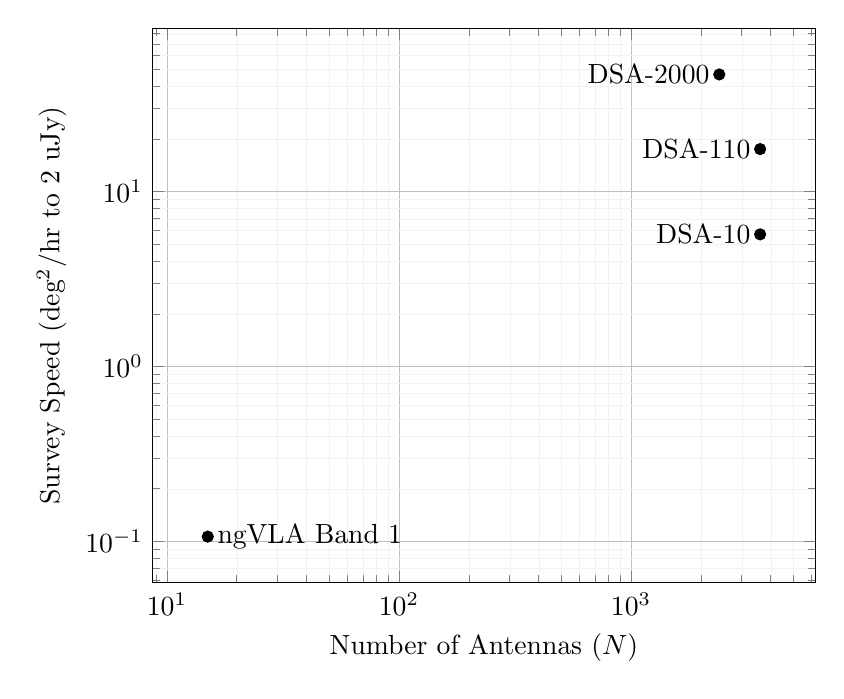
\begin{tikzpicture}[
        declare function={
        Lambd(\F) = \CZ/\F;
        SS(\TSYS,\D,\ETAA,\B,\N,\F) = 1.217 * \ETAA * \B * (Lambd(\F)*\SNU*\N*\D/\TSYS)^2;
            %CostDSA10(\N) = 10e3*\N + 5*\N^2; % $100M @ N=3600
            %Cost(\N) = 30e3*\N + 5*\N^2;       % $100M @ N=2400
            %CostCold(\N) = 130e3*\N + 5*\N^2;  % $100M @ N=80
            %CostngVLA(\N) = 7e6*\N + 5*\N^2;  % $100M @ N=15
        },
    ]
        \newcommand\CZ{299792458}
        \newcommand\SNU{2e-6}
        
        \begin{axis}[width={10cm}, 
                    grid={both}, 
                    grid style={line width={.1pt}, 
                    draw={gray!10}},
                    ymode=log,
                    xmode=log,
                    major grid style={line width={.2pt}, draw={gray!50}},
                    legend pos={south east},
                    ylabel={Survey Speed (deg$^2$/hr to 2 uJy)},
                    xlabel={Number of Antennas ($N$)}]
            % DSA-110
            \addplot[samples at={3600},only marks]{SS(25,4.65,0.7,250e6,x, 1.4e9)} node[left]{DSA-110};
            % DSA-10
            \addplot[samples at={3600},only marks]{SS(60,4.5,0.7,500e6,x, 1.4e9)} node[left]{DSA-10};
            % DSA-2000
            \addplot[samples at={2400},only marks]{SS(25,5,0.7,1.3e9,x, 1.4e9)} node[left]{DSA-2000};
            % % DSA-2000 W/Cryo
            % \addplot[samples at={80},only marks]{SS(18,5,0.7,1.3e9,x, 1.4e9)} node[right]{DSA-2000 w/ Cryo};
            % ngVLA Band 1
            \addplot[samples at={15},only marks]{SS(17.07,18,0.828,2.3e9,x, 1.4e9)} node[right]{ngVLA Band 1};
        \end{axis}
    \end{tikzpicture}
\end{document}